\section{Spatial Operations}
\label{sec:query}
\name introduces new {\em physical execution plans} inside Spark SQL
for spatial operations. In particular, the support for local and
global indexes enables \name to explore many efficient implementations
of classic spatial operations in the context of Spark. In this
section, we will discuss four operators as representatives for spatial
queries and analytics in \name, namely, range query, k nearest
neighbor ($\knn$) query, distance join, and $\knn$ join.

\subsection{Range Query}
\label{sub:range}
Two types of range queries are supported in \name. They differ by the
shape used to specify the query area, which is either a rectangular
box or a circle, leading to box and circle range query
respectively. Intuitively, these range queries can be expressed and
treated as standard SQL queries in Spark SQL, using filters with
properly constructed range conditions. However, without using \name's
query interface introduced in Section \ref{sec:parser}, the expression
becomes clumsy and error prone. And more importantly, without indexes,
the query evaluation will have to scan all records in the table, which
is very inefficient and resource intensive.

In contrast, \name allows users to express both range queries
natively as shown in Section \ref{sec:parser}, and it can handle range
queries using index (assume that the spatial attributes are indexed):

% \begin{figure}[t!]
% 	\centering
% 	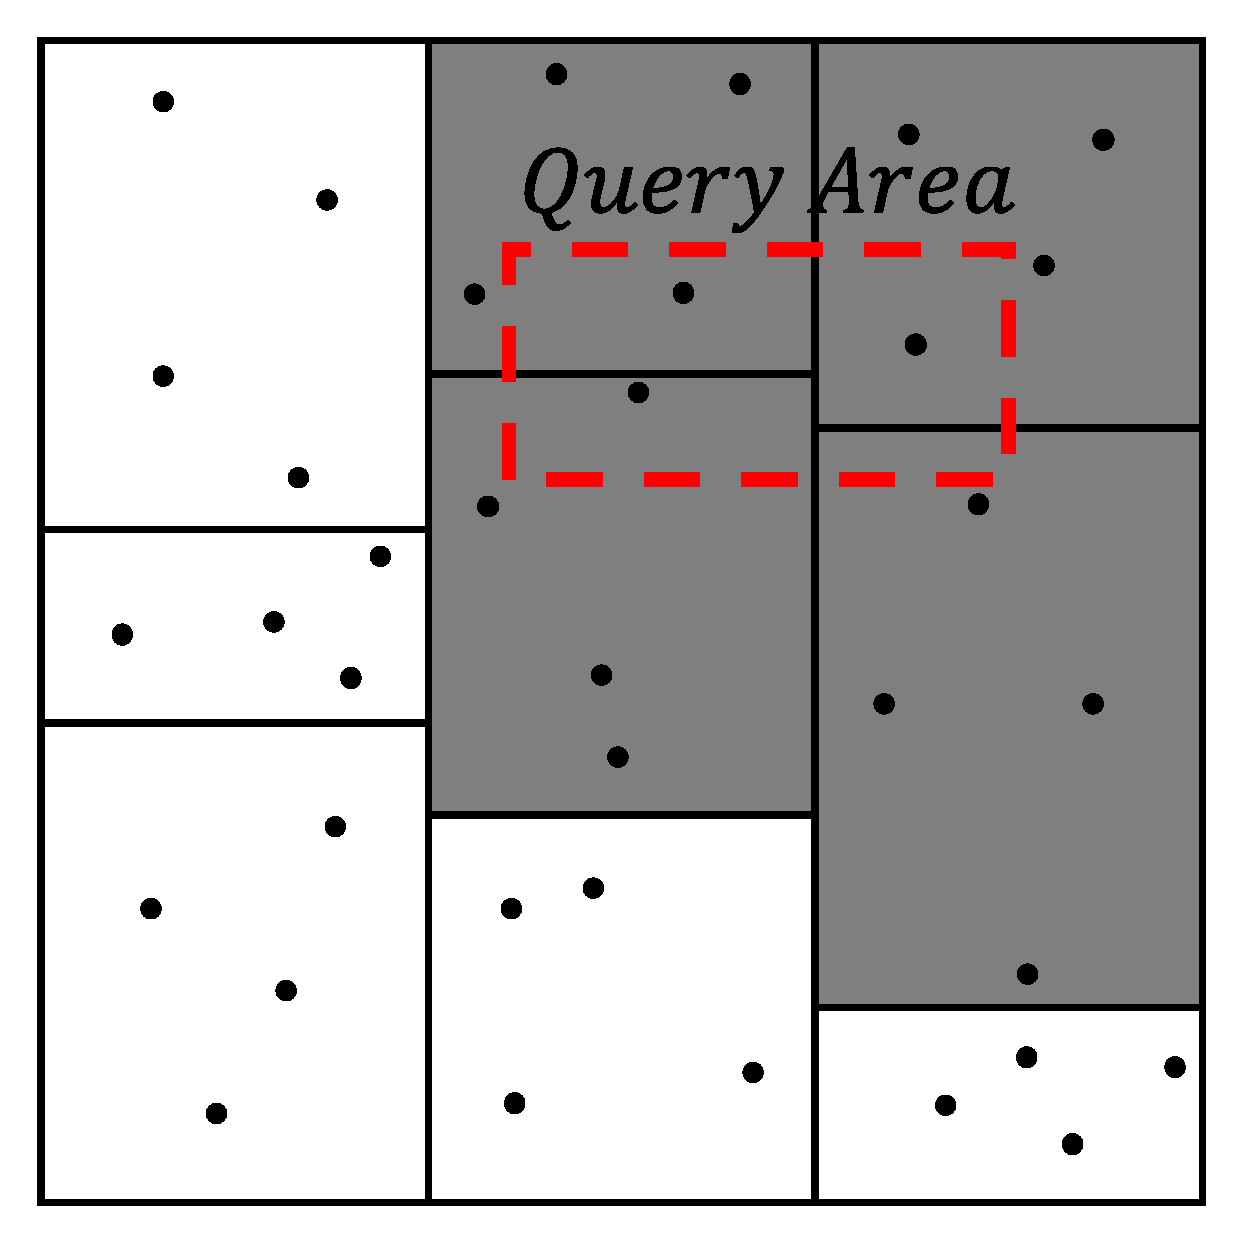
\includegraphics[width = 1.55in]{figs/range}
% 	\vspace{-4mm}
% 	\caption{Range Query}
% 	\label{fig:oprange}
%     \vspace{-3mm}
% \end{figure}


\Paragraph{Global filtering.} In this step, \name uses the global
index to prune partitions that do not overlap with the query range. In
particular, \name inspects the global index to obtain ids of the
partitions which intersect the query area. Next, \name calls
\texttt{PartitionPruningRDD}, a Spark internal developer API that
filters partitions by ID, to mark required partitions.

\Paragraph{Local processing.} On selected partitions from global
filtering, \name processes them in parallel. For each partition, \name
exploits its local index to quickly return matching records from the
local array. Note that if $\mbr(R_i)$ is completely inside the query
area, all records in $R_i$ can be returned without even checking the
index. In general, local index helps reduce query cost over $R_i$
significantly compared to scanning $R_i$ entirely in Spark SQL.

% For instance, in Figure \ref{fig:oprange}, we first query the global
% index to find all partitions whose regions intersect the query area
% (shaded area in the figure). Then, \SparkSpatial invokes a range query
% on the local index of each selected partitions to get the final
% results.
\subsection{kNN Query}
\label{sub:knn}
Using Spark SQL, a $k$NN query can be processed in two steps: (1)
calculate distances from all points in the table to the query point;
(2) take $k$ records with minimum distances. This procedure can be
naturally expressed as an RDD action \texttt{takeOrdered}, where users
can specify a comparison function and a value $k$ to select $k$
minimum elements from RDD. However, this solution invokes distance
computation for every record, a top $k$ selection on each RDD
partition, and shuffling of large intermediate results.

In \name, $k$NN queries achieve much better performance by utilizing
indexes. It leverages two observations: (1) once at a local partition,
fast $k$NN selection over the local data is possible using the local
index; (2) a tight pruning bound that is sufficient to cover the
global $k$NN results can be used for pruning at the global index. The
first observation is a simple application of classic $k$NN query
algorithms using spatial index like R-tree
\cite{DBLP:conf/sigmod/RoussopoulosKV95}. The second observation
deserves some discussion.
\begin{figure}[htb]
	\subfigure[Loose Pruning Bound]{
		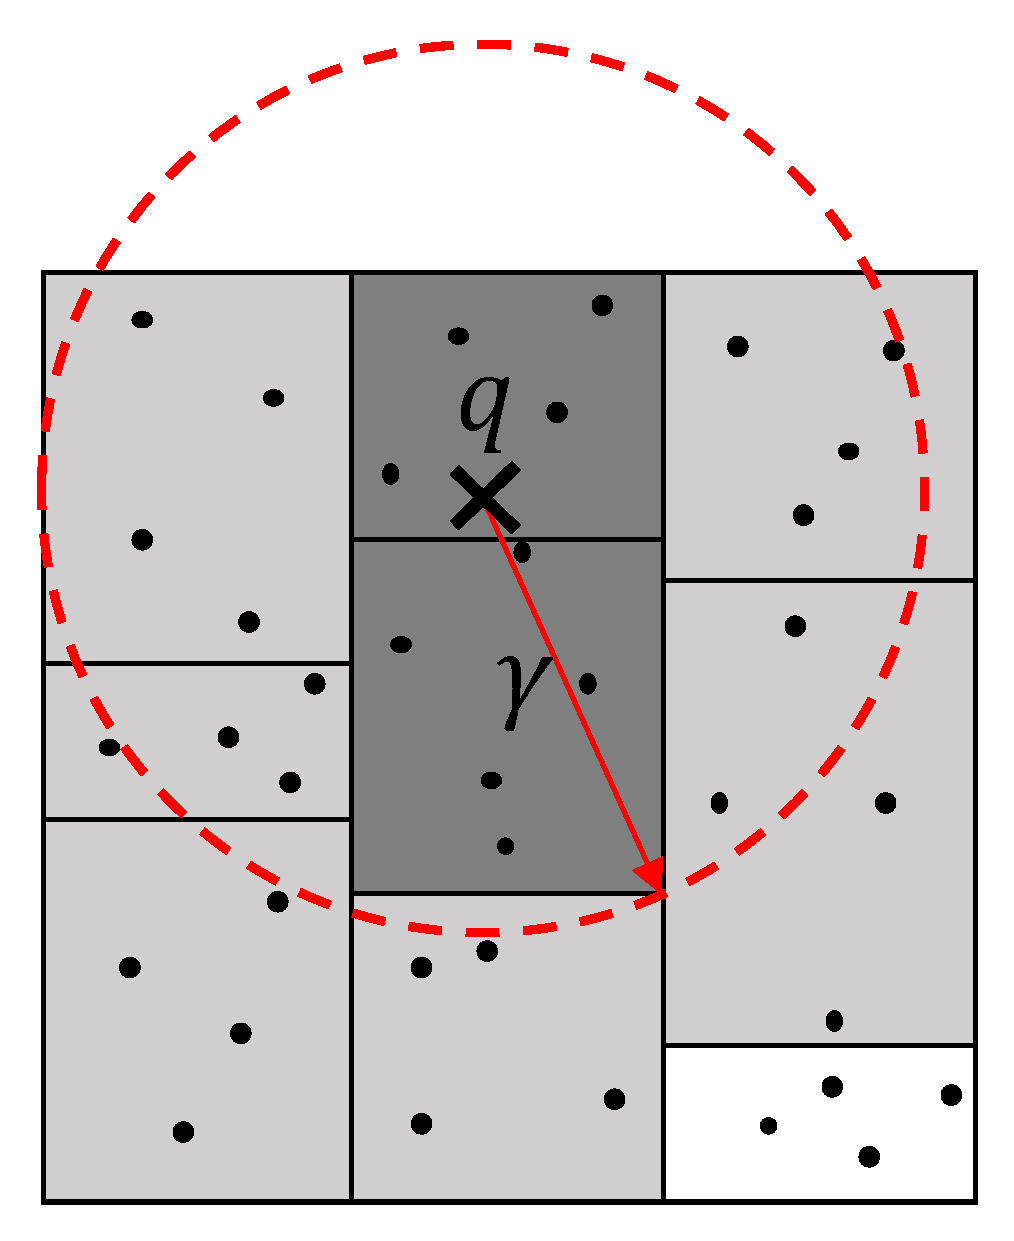
\includegraphics[width=1.55in]{figs/knnbound1}
		\label{fig:knnbound1}}
	\subfigure[Refined Pruning Bound]{
		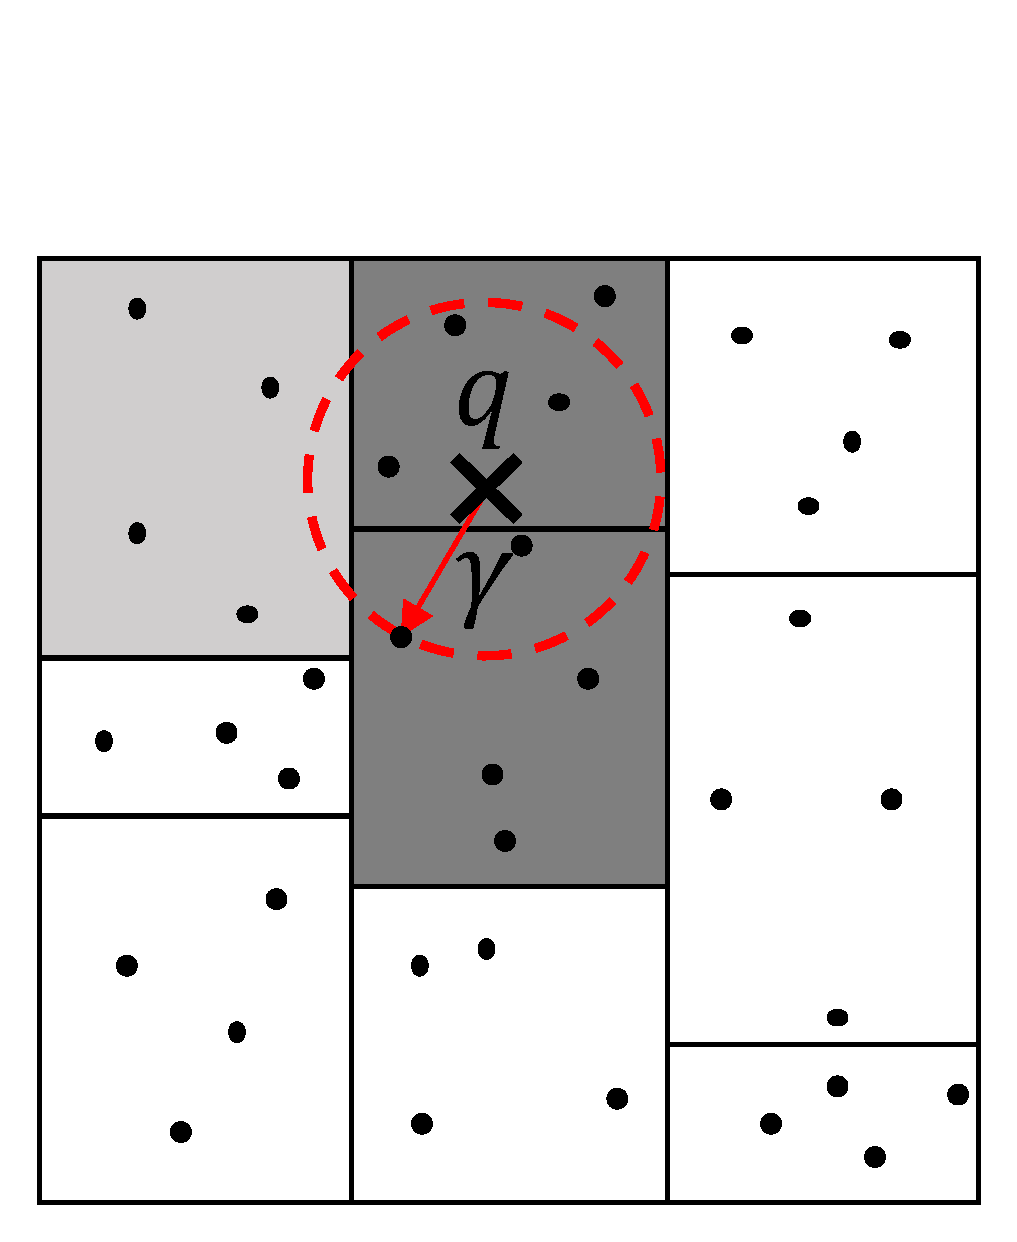
\includegraphics[width=1.55in]{figs/knnbound2}
		\label{fig:knnbound2}}
	\caption{Pruning bound for $k$NN query at global index.}%\vspace{-1mm}
	\label{fig:knnbound}
\end{figure}

Intuitively, any circle that centers at the query point $q$ and covers
at least $k$ points from $R$ is a safe bound for pruning. To generate
a tight pruning bound, we need to shrink the radius $\gamma$ of this
circle. A loose pruning bound can be obtained using the global index.
We find the nearest partition(s) to the query point $q$, that are
sufficient to cover at least $k$ data points; retrieve more than one
partitions if the nearest partition does not have $k$ points (note
that global index maintains the counts for the number of records in
each partition). The distance between $q$ and a partition $R_i$ is
defined as $\maxdist(q, \mbr(R_i))$
\cite{DBLP:conf/sigmod/RoussopoulosKV95}. Without loss of generality,
assume the following MBRs are returned:
$\{\mbr(R_1), \ldots, \mbr(R_\ell)\}$.  Clearly,
$\gamma=\max\{\maxdist(q, \mbr(R_1)), \ldots, \maxdist(q, R_\ell)\}$
is a safe pruning bound. Figure \ref{fig:knnbound1} shows an example
of this bound as a circle centered at $q$. The dark boxes are the
nearest MBRs retrieved to cover at least $k$ points which help derive
the radius $\gamma$. The dark and gray boxes with shadows are
partitions selected by the global index according to this pruning
bound.

To tighten the pruning bound, \name issues a $k$NN query on the $\ell$
partitions selected from the first step (i.e., two partitions with
dark boxes in Figure \ref{fig:knnbound1}), and takes the $k$-th
minimum distance from $q$ to the $k\ell$ candidates returned from
these partitions as $\gamma$.  Figure \ref{fig:knnbound2} shows this
new pruning bound which will be much tighter in practice. Note that
$\ell$ is small for typical $k$ value (often $\ell=1$), thus, this
step has very little overhead.

Global index returns the partition ids whose MBRs intersect with the
circle centered at $q$ with radius $\gamma$, \name marks these
partitions using \texttt{PartitionPruningRDD} and invokes local $k$NN
queries using the aforementioned observation (1). Finally, it merges
$k$ candidates from each such partition and takes the $k$ records with
minimum distance to $q$ using RDD action \texttt{takeOrdered}.

\subsection{Distance Join}
\label{sub:disjoin}
Distance join is a $\theta$-join between two tables. Hence, we can
express a distance join $R \Join_{10.0} S$ in Spark SQL as:
\begin{lstlisting}[language=SQL]
SELECT * FROM R JOIN S
ON (R.x - S.x) * (R.x - S.x) + (R.y - S.y) * (R.y - S.y)
     <= 10.0 * 10.0
\end{lstlisting}\vspace{-2mm}

Spark SQL will have to use the cartesian product of two input tables
to process $\theta$-joins.  It filters rows from the cartesian product
based on the given predicates. Producing and scanning through
the cartesian product is rather costly in Spark, since it is based on
broadcasting the partitions and if two tables are roughly the same
size, this leads to $O(n^2)$ cost if each table has $n$ partitions.

Note that most existing systems we reviewed in Section
\ref{sec:background} have not studied distance join; rather, they
studied {\em spatial join}. A {\em spatial join} takes two tables $R$
and $S$ (each is a set of spatial objects expressed as some geometric
objects such as polygons), and a spatial join predicate $\theta$
(e.g., \texttt{overlaps}, \texttt{contains}) as input, and it returns
the set of all pairs $(r, s)$ where $r \in R$, $s \in S$ such that
$\theta(r, s)$ is true; $\theta(r,s)$ is evaluated as object $r$
`$\theta$' (e.g, overlaps) object $s$.  

That said, we design the \emph{DJSpark} algorithm in \name for
distance joins.  DJSpark consists of three steps: data partition,
global join, and local join, as shown in Figure \ref{fig:sjmrdis}.

\Paragraph{Data partition.} The main objective of data partition phase
is to partition $R$ and $S$ so that spatial locality is preserved and
records that are close to each other (from both $R$ and $S$) will end
up in the same corresponding partitions. Besides, we also need to
consider partition size (so data from two corresponding partitions
from $R$ and $S$ respectively can both fit in memory) and load
balancing issues. Therefore, we can re-use the \emph{STRPartitioner}
introduced in Section \ref{sec:index} as the partitioner. The main
difference is how we decide the partition size for $R$ and $S$. \name
needs to ensure that it can keep two partitions (one from $R$ and one
from $S$) rather than one (when handling single-relation operations like
range queries) in executors' heap memory space at the same time. 

Note that the data partition phase can be skipped for $R$ (or $S$) if
$R$ (or $S$) is already indexed.

\Paragraph{Global join.} Given the partitions for tables $R$ and $S$,
this step produces all pairs $(i, j)$'s which may contribute any pair
$(r, s)$, such that $r\in R_i$, $s\in S_j$, and $|r, s|\le \tau$.
Observe that each record in $s\in S$, $s$ matches with some records in
$R_i$ {\em only if} $\mindist(s, R_i)\le \tau$. We can generalize to
produce the pairs $(i, j)$'s such that \name only checks them if
$\mindist(R_i, S_j)\le \tau$. After generating these candidate pairs
of partition ids, \name produces a single partition $P=\{R_i, S_j\}$
for each pair $(i, j)$ and these partitions are sent to workers for
processing local joins in parallel.

\Paragraph{Local join.} Given a partition $P=\{R_i, S_j\}$ produced by
the global join, local join builds a local index over $S_j$ on the fly
(if $S$ is not already indexed). For each record $r\in R_i$, \name
finds all $s\in S_j$ such that $|s, r|\le \tau $ using $r$ over the
local index on $S_j$.

\begin{figure}
	\centering
	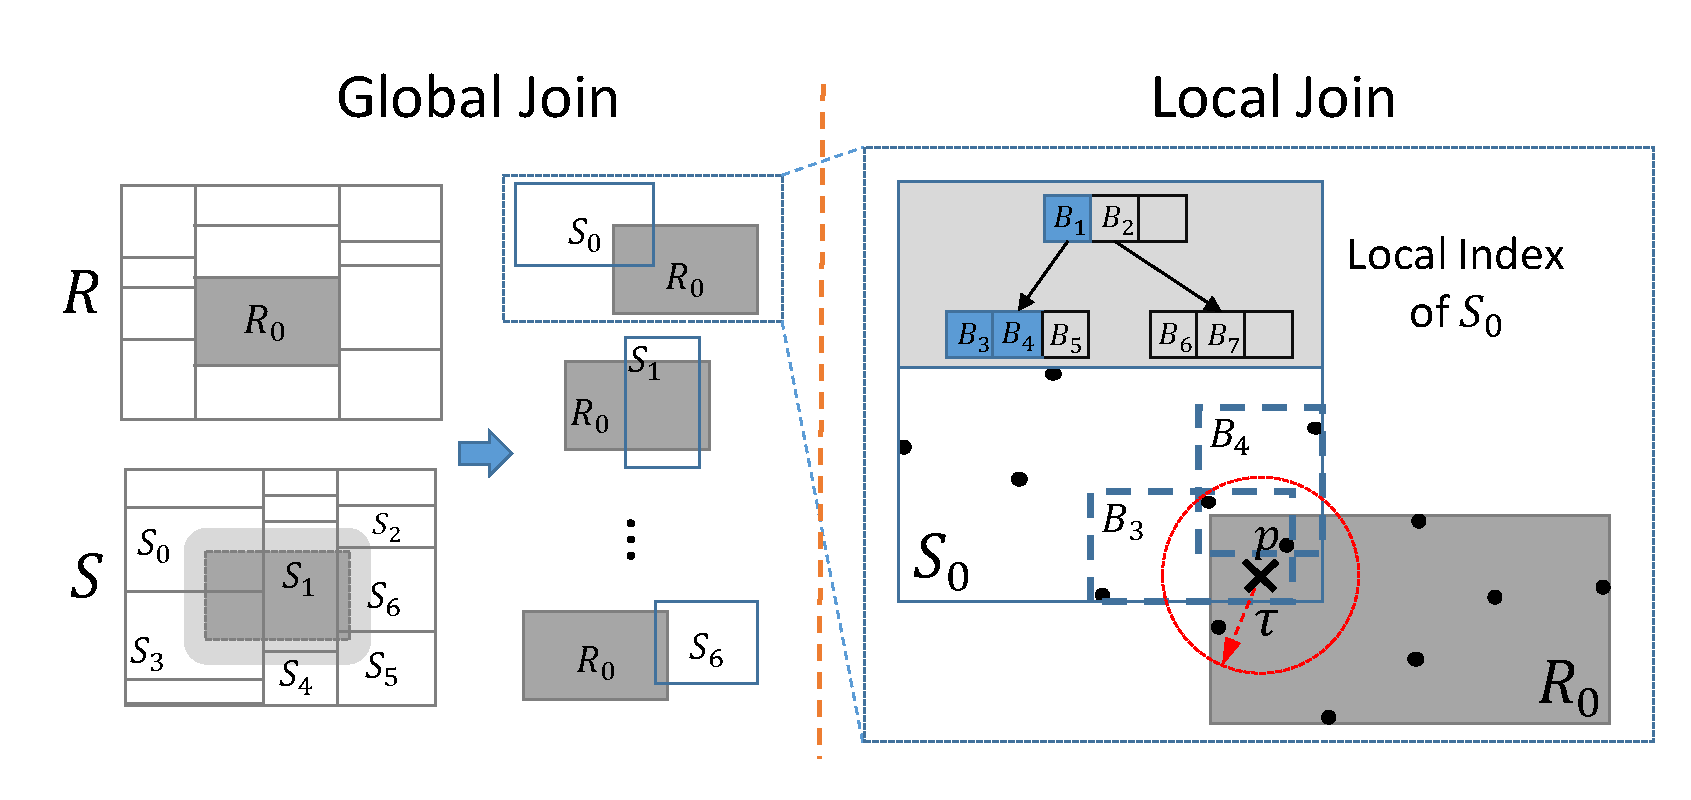
\includegraphics[width = 3.4in]{figs/SJMR-DIS}
	\vspace{-8mm}
	\caption{The DJSpark algorithm in \name.}
	\label{fig:sjmrdis}\vspace{-4mm}
\end{figure}

% For distance joins whose matched record number is not too large,
% \SarkSpatial provides an alternative approach (termed as R-Tree
% distance join) similar to distributed hash join. Instead of finding
% all matched partition pairs in the second step described above, we
% duplicate each record in $S$ as a matching candidate of $P_R^i$ if its
% minimum distance to $A_R^i$ is less than $rd$. To get the final
% result, \SparkSpatial combines $P_R^i$ with all its matching
% candidates in a partition and invokes a local join on each combined
% partition to get the final result. This algorithm avoids data
% partitioning on $S$ and reduces record duplication as duplication
% granularity is on record level rather than partition level. However,
% when $rd$ is getting larger, sizes of the combined partitions will
% grow drastically and finally cause memory overflow.

\subsection{kNN Join}
\label{sub:knnjoin}
Several solutions \cite{bcknnj, feifeiknnj} for $k$NN join have been
proposed in the MapReduce framework. \name has redesigned and
implemented these methods with the RDD abstraction of
Spark. Furthermore, \name designs a new simple hash-join like
algorithm based on the STR partitioning strategy and its R-tree index,
which shows the best performance in Spark. % We will briefly describe
% the the adaption of existing methods into \name, and introduce our new
% algorithm RKJSpark.

\subsubsection{Baseline methods}
\label{subsub:bnlj}
The most straightforward method is to adopt the block nested loop
methodology \cite{feifeiknnj}. We dub this method \emph{BKJSpark-N}
(block nested loop $k$NN join in Spark).

\Paragraph{Producing buckets.} $R$ (and $S$) is divided into $n_1$
($n_2$) equal-sized blocks, which simply puts every $|R|/n_1$ (or
$|S|/n_2$) records into a block. Next, every pair of blocks, i.e.,
$(R_i, S_j)$ for $i\in[1, n_1], j\in [1, n_2]$ are shuffled to a
bucket (so a total of $n_1n_2$ buckets). % \name uses \texttt{flatmap}
% over each record $r$ to assign a bucket number for $r$.  A partitioner
% is implemented to partition RDDs according to these bucket
% numbers. The values of $n_1$ and $n_2$ are determined based on the
% memory size of worker nodes and the size of the input relation.

\Paragraph{Local $k$NN join.} Buckets are processed in
parallel. Within each bucket $(R_i, S_j)$, \name performs
$\knn(r, S_j)$ for every $r\in R_i$ though a nested loop over $R_i$
and $S_j$. % The result for each record
% $r \in R$ is passed to next step in form $(r, list(s, |r, s|))$ where
% the list stores local $k$NN of $r$.

\Paragraph{Merge.} This step finds the global $k$NNs for every
$r \in R$ among its $n_2$ local $k$NNs found in the last step (a total
of $nk$ candidates). \name runs \texttt{reduceByKey} (where key is a
record in $R$) in parallel to get the global $k$NNs for each record
record in $R$.

A simple improvement is to build a local R-tree index over $S_j$ for
every bucket $(R_i, S_j$) and use the R-tree for local $k$NN joins,
which is denoted as \emph{BKJSpark-R} (block R-tree $k$NN join in Spark).

% the records from $S$ in each bucket, which accelerates finding $k$NN
% of a record $r \in R$ in the same bucket. Specifically, for each
% partition $P_S^i$ ($1 \leq i \leq n$), we bulk load a local spatial
% index, in particular we use R-Tree, before proceeding to find local
% $k$NN of each record from $R$ in the same bucket. Then, we use the
% $k$NN functionality provided by R-Tree to answer $kNN(r, P_S^i)$ in
% every bucket. Note that both R-Tree bulk loading and $k$NN search in
% R-Tree are very efficient. Hence, this overhead is compensated by
% savings from not running a local nested loop in each bucket. Applying
% this improvement, we dub it \emph{S-BRJ} (Spark Block R-Tree Join)

\subsubsection{Voronoi $k$NN Join and $z$-Value $k$NN Join}
\label{subsub:voronoi}
The baseline methods needs to check roughly $n^2$ buckets (if
$O(n_1)=O(n_2)=O(n)$) which is expensive for both computation and
communication in distributed systems. A MapReduce algorithm leveraging
a Voronoi diagram based partitioning strategy was proposed in
\cite{bcknnj}, which executes only $n$ local joins by partitioning
both $R$ and $S$ into $n$ partitions respectively. The partition
strategy is based on the voronoi diagram for a set of pivot points
selected from $R$ and we refer interested readers to \cite{bcknnj} for
further details. We have adapted this approach in \name, denoted as
the VKJSpark method (voronoi $k$NN join in Spark).

Another MapReduce based algorithm for $k$NN join was proposed in
\cite{feifeiknnj} that explores $z$-values to map multi-dimensional
points into one dimension and uses {\em random shift} to preserve
locality. This approach is also able to produce $n$ partitions for $R$
and $S$ respectively, such that for any $r\in R_i$ for $i\in [1, n]$,
$\knn(r, S)\subseteq \knn(r, S_i)$ {\em with high probability}. Thus,
it is able to produce high quality approximations using only $n$ local
joins. The partition step in this approach is simpler than the
aforementioned voronoi-based method, but it only provides approximate
results by default and there is an added cost for producing exact
results in a post-processing step. We have adapted this approach too
in \name and denote it as ZKJSpark ($z$-value $k$NN join in Spark).


% The basic idea is to generate a small set of random samples from
% $R$, known as the pivot points and denoted as $P$. The voronoi
% diagram of $P$ is constructed; suppose $|P|=n$ and its voronoi
% diagram naturally has $n$ voronoi cells. $R$ is partitioned into $n$
% {\em disjoint partitions} $R_1, R_2, \cdots, R_n$, such that $R_i$
% are fully contained by the $i$th voronoi cell for the $i$th pivot
% $p_i\in P$. Next, $S$ is partitioned into $n$ partitions $\{S_1,
% \ldots, S_n\}$ {\em that may overlap}, such that $S_i\subset S$ and
% $\forall r\in R_i$, $\knn(r, S)\subseteq S_i$. Note that there are
% many different partitions $\{S_1, \ldots, S_n\}$ that will satisfy
% the above condition (e.g., in the extreme case, we can simply set
% $S_i=S$ for all $i\in[1,n]$), the method in \cite{bcknnj} leverages
% points in $\knn(p_i, S)$ and points in $R_i$ to derive a good
% partition of $S$. We refer interested readers to \cite{bcknnj} for
% further details.



% This approach avoids duplication on table $R$ and sending entire set
% $S$ to all executors. Yet, to guarantee the correctness of $k$NN join,
% subset $S_i$ must contains $k$NN of every $r \in P_R^i$ (i.e.
% $\forall r \in P_R^i, kNN(r, S) \subset S_i$). Note that
% $S_i \cap S_j$ may not be empty, as it is possible that an object $s$
% is one of the $k$NN of $r_i \in P_R^i$ and $r_j \in P_R^j$. Therefore,
% some records from $S$ will be duplicated and distributed to multiple
% executors. Obviously, if we can reduce the average number of
% duplications for objects in $S$, both shuffling and computational cost
% can be reduced, which makes it a key optimization goal.

% Generally, Voronoi $k$NN join runs in three stages shown as following:

% \Paragraph{1. Preprocessing.} The preprocessing step finds out a set
% of pivot objects based on input table $R$. These pivots are used to
% create a Voronoi diagram, which can help partition records in $R$
% effectively while preserving their proximity. In \SparkSpatial, we
% take a random selection strategy to select pivots, in which $T$ random
% sets are selected from $R$ and the set with maximum sum distance
% between every two points is selected as the pivot set for data
% partitioning.

% \Paragraph{2. Data Partitioning.} This stage takes selected pivots and
% tables $R$ and $S$ as input. It finds out the nearest pivot for each
% record in $R \cup S$ and computes the distance between the record and
% the pivot. The result of this stage is a partitioning on $R$ and $S$,
% based on the Voronoi diagram of the pivots. Meanwhile, we also collect
% some statistics about each partition of $R$ and $S$. In \SparkSpatial,
% \texttt{VoronoiPartitioner} is defined to partition tables according
% to a set of pivots. Besides, we make use of RDD operation
% \texttt{mapPartitions} to get partition statistics.

% \Paragraph{3. Local $k$NN Join.} Given the partitioning on $R$, this
% stage first finds the subset $S_i$ for each partition $P_R^i$ based on
% the statistics collected in the last step. Specifically, we calculate
% a lower bound for $P_S^j$ against each $P_R^i$.\footnote{Please refer
%   to \cite{bcknnj} for more details about how to calculate such lower
%   bound.} Record in $P_S^j$ whose distance to the partition pivot is
% greater than the lower bound for $P_R^i$ will be duplicated as an
% element in $S_i$. Finally, \SparkSpatial uses \texttt{zipPartitions}
% to combine each pair of $P_R^i$ and $S_i$ and performs a local $k$NN
% join to get the final answer.

% \Paragraph{Improvement: Geometric Grouping.} Intuitively, by selecting
% a larger number of pivots, we can split input tables into a set of
% Voronoi cells (corresponding to partitions) with finer
% granularity. This will make the lower bounds calculated in step 3
% tighter. However, this will cause an explosion on the number of local
% $k$NN join tasks, which may result in terrible overall performance due
% to numerous scheduling and shuffling costs. Moreover, partitions
% generated by Voronoi diagram partitioning strategy suffer from serious
% load balancing issue. To address these problems, a natural idea is to
% divide Voronoi cells into disjoint groups and partition data according
% to these groups. Following the experimental results presented in
% \cite{bcknnj}, \SparkSpatial picks Geometric Grouping algorithm as
% grouping strategy, in which we divide Voronoi cells whose pivots are
% near to each other into the same group.\footnote{Please refer to
%   \cite{bcknnj} for more details of Geometric Grouping algorithm.}

\subsubsection{R-Tree $k$NN Join}
\label{subsub:rtknnj} 
We leverage the indexing support in \name to design a simpler yet more
efficient $k$NN join method, the RKJ-Spark method (R-tree $k$NN join
in Spark).

RKJ-Spark partitions $R$ into $n$ partitions $\{R_1, \ldots, R_n\}$
using the STR partitioning strategy, as introduced in Section \ref{sec:index},
which leads to balanced partitions of $R$ and preserves the locality
as well. It then takes a set of random sample $S'$ from $S$ and build
a R-tree index $T$ over $S'$ in the driver program on the master node.

% \begin{figure}
%   \subfigure[\small Bound centers at $\forall r \in R_i$]{
% 		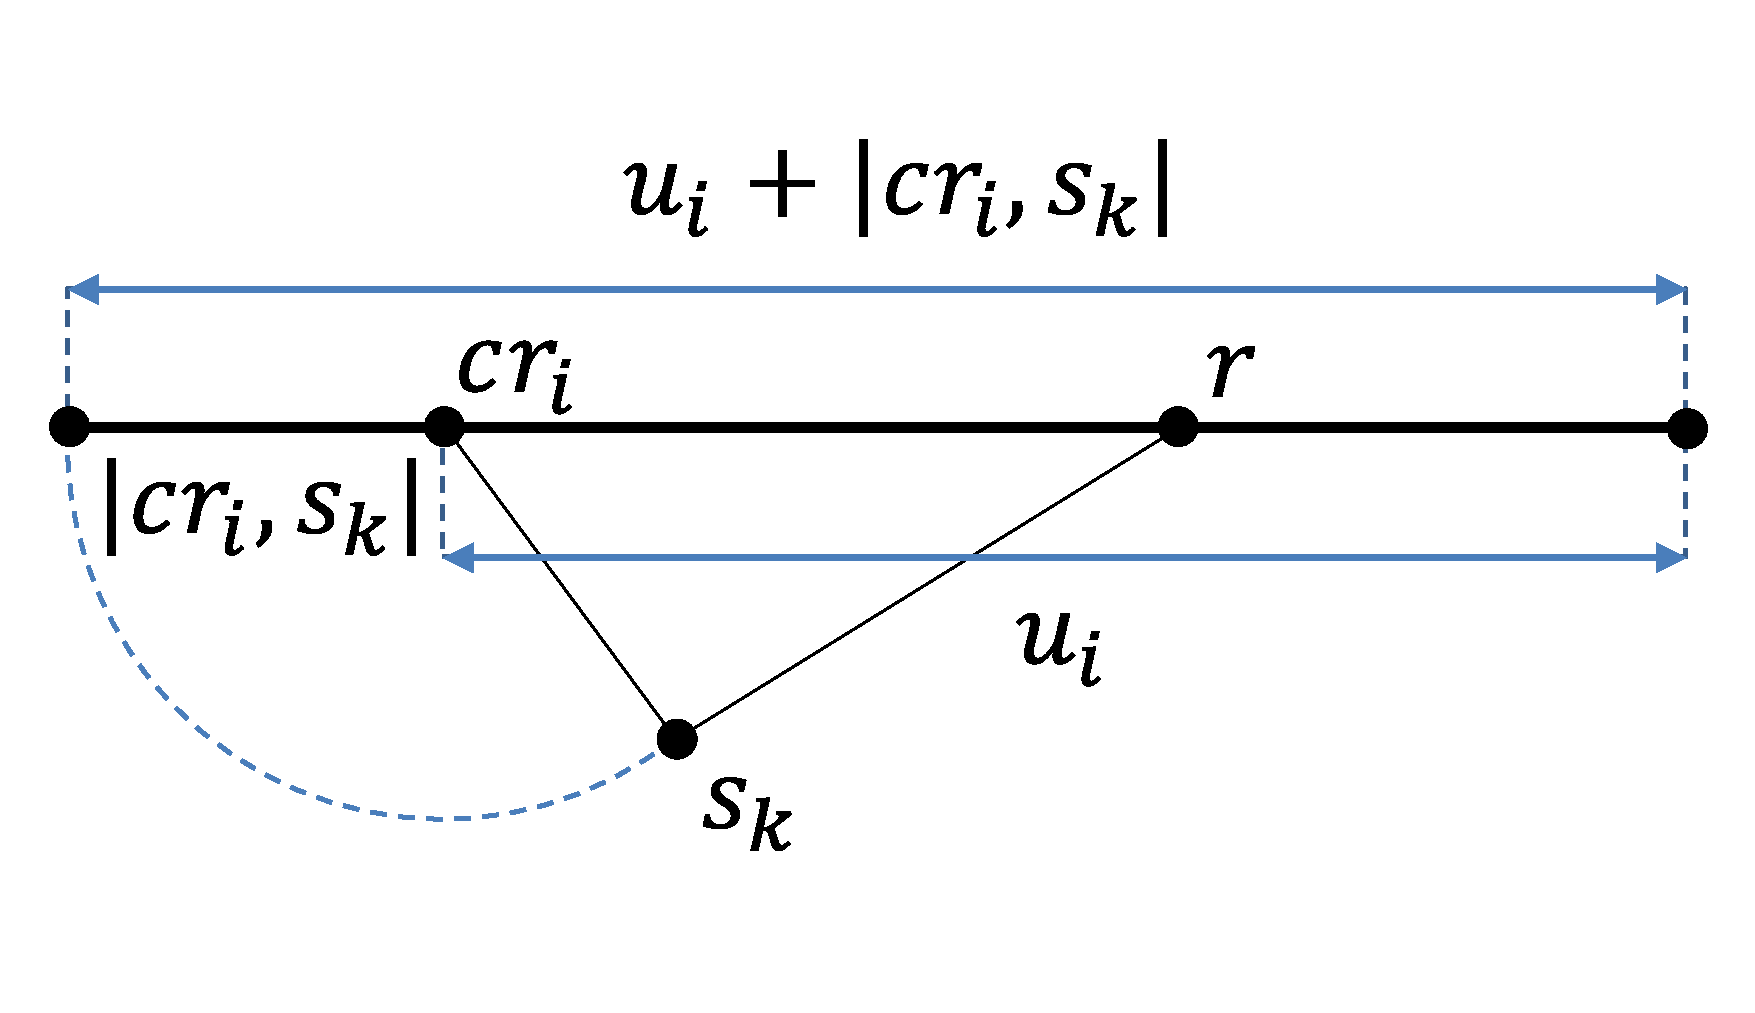
\includegraphics[width=1.6in]{figs/knnjbound1}
% 		\label{fig:knnjbound1}}
% 	\subfigure[\small Bound centers at $cr_i$]{
% 		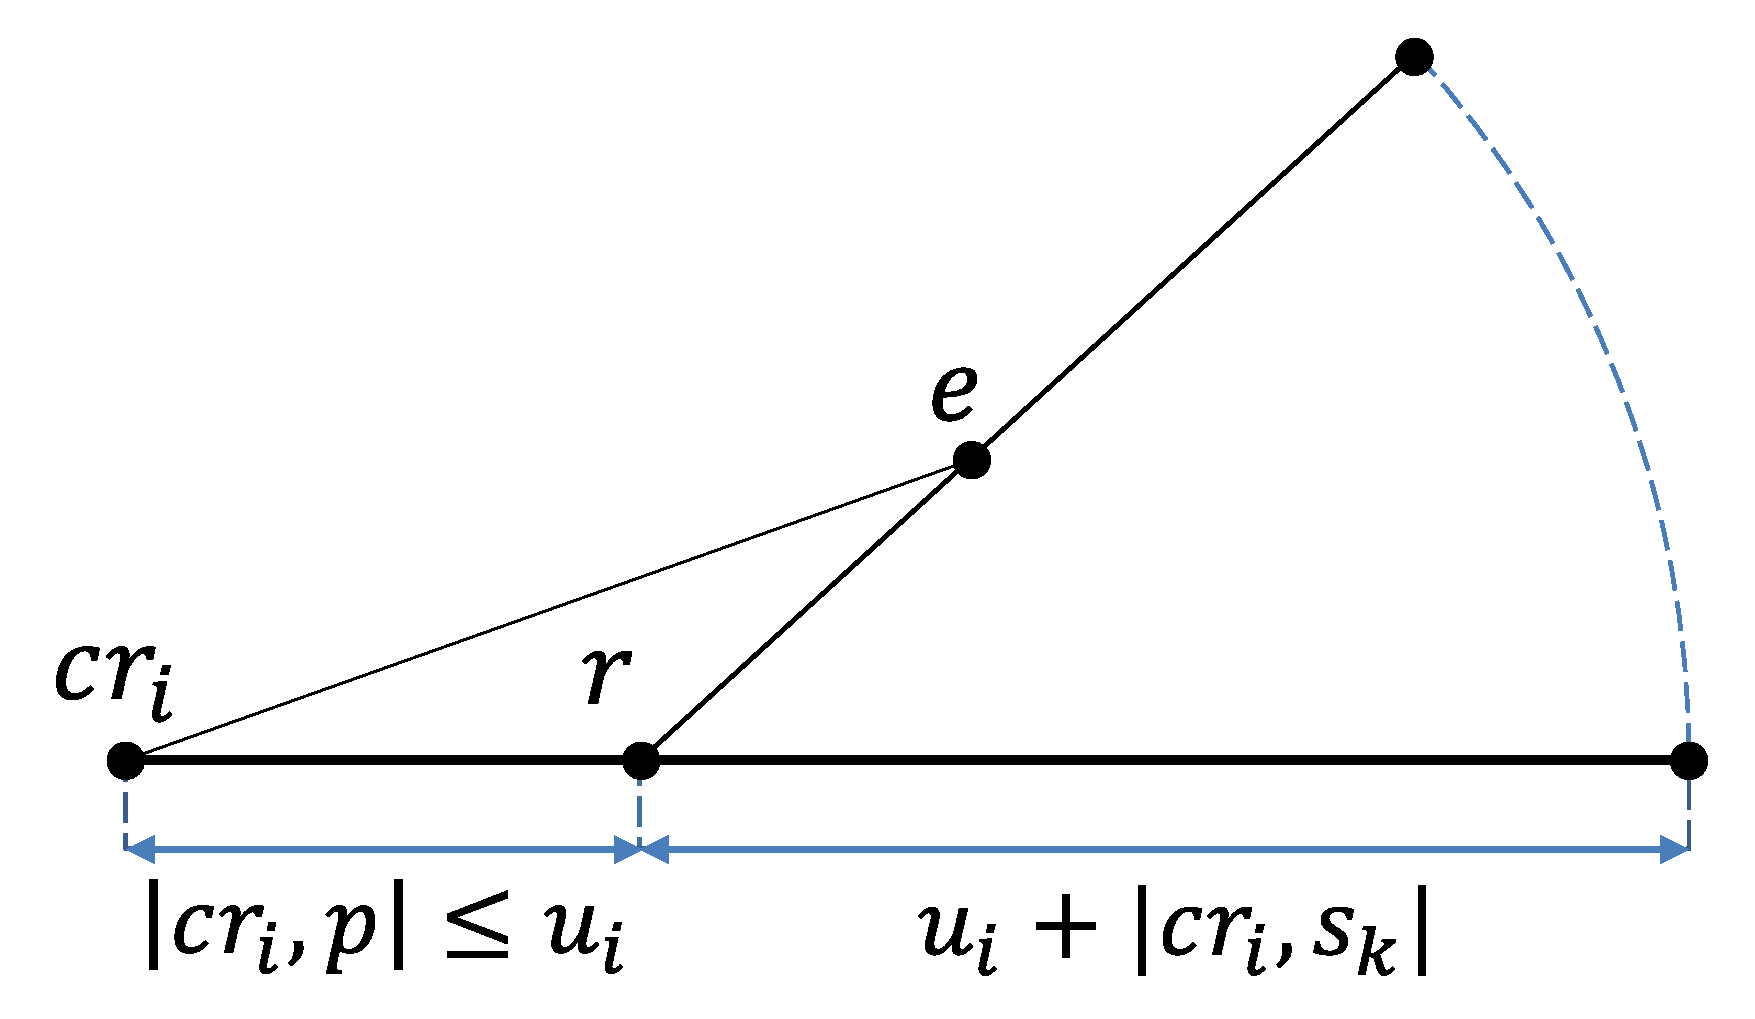
\includegraphics[width=1.6in]{figs/knnjbound2}
% 		\label{fig:knnjbound2}}
%       \caption{Distance bound for RKJ-Spark.}\vspace{-4mm}
% 	\label{fig:knnjbound}
% \end{figure}

The key idea in RKJ-Spark is to derive a distance bound $\gamma_i$ for
each $R_i$, such that we can use $\gamma_i$, $R_i$, and $T$ to find a
subset $S_i\in S$ so that for any $r\in R_i$, $\knn(r, S)=\knn(r,
S_i)$. This partitioning strategy ensures that $R \Join_{\knn} S =
(R_1 \Join_{\knn} S_1) \bigcup (R_2 \Join_{\knn} S_2)\bigcup \cdots
\bigcup (R_n \Join_{\knn} S_n)$, and allows the parallel execution of
only $n$ local $k$NN joins (every $(R_i, S_i)$ pair for $i\in[1, n]$)).


We use $cr_i$ to denote the centroid of $\mbr(R_i)$. First, in
parallel for each $R_i$, \name finds the distance $u_i$ from the
furthest point in $R_i$ to $cr_i$, i.e., $u_i=\max_{r\in R_i}|r,
cr_i|$. \name sends these $u_i$ values and centroids back to the
master node.

Next, the driver program on the master node finds $\knn(cr_i, S')$
using the R-tree $T$ for $i\in[1, n]$. Without loss of generality,
suppose $\knn(cr_i, S')=\{s_1, \ldots, s_k\}$ (in ascending order of
their distances to $cr_i$). Finally, \name simply sets:
\begin{equation}
\label{eq:rkjbound}
 \gamma_i= 2u_i +|cr_i, s_k| \textrm{ for partition $R_i$},
\end{equation}
and finds $S_i=\{s|s \in S, |cr_i, s|\leq \gamma_i\}$ using a circle
range query centered at $cr_i$ with radius $\gamma_i$ over $S$. This
guarantees the desired property as described above, due to:
\vspace{-3mm}
\begin{theorem}
\label{thm:rtknnj}
For any partition $R_i$ where $i \in[1, n]$, we have:
\[\forall r \in R_i, \knn(r, S) \subset \{s|s \in S, |cr_i, s| \leq
\gamma_i\},  \textrm{ for }\gamma_i \textrm{ defined in }\eqref{eq:rkjbound}.\]
\end{theorem}
The proof is shown in Appendix \ref{sec:proof1}.  This leads to the
design of RKJ-Spark. Specifically, for every $s \in S$, RKJ-Spark
includes a copy of $s$ in $S_i$ if $|cr_i, s| \leq \gamma_i$. Theorem
\ref{thm:rtknnj} guarantees that for any $r\in R_i$, $\knn(r,
S)=\knn(r, S_i)$.

Thus, \name invokes a \texttt{zipPartitions} operation for each
$i\in[1, n]$ to place $R_i$ and $S_i$ together into one RDD
partition. In paralle, on each such RDD partition, \name builds a
R-tree over $S_i$ and executes a local $k$NN join using $R_i$ over
this tree. The union of these $n$ outputs is the final answer for
$R\Join_{\knn}S$.

%Though sharing basic ideas with Voronoi $k$NN join, R-Tree $k$NN join
%requires less computations when partitioning input tables and
%calculating distance bounds. Besides, it avoids geometric grouping
%which is used to keep load balance and control the number of local
%$k$NN join tasks. Generally speaking, compared with Voronoi $k$NN join,
%R-Tree $k$NN join is much easier to implement and achieves comparable
%performance as well (see experiment results in Section \ref{sec:exp}).


%%% Local Variables:
%%% mode: latex
%%% TeX-master: "paper"
%%% End:
